\documentclass[12pt]{article}
\usepackage{geometry}
\usepackage{booktabs}
\usepackage{longtable}
\usepackage{hyperref}
\usepackage{graphicx}
\geometry{margin=2.5cm}
\usepackage{float}

\begin{document}

\section{Test of different Huggingface models}

\subsection{Data preparation and selection}
I took all the messages and kept those annotated, I balanced the number of BULLISH/BEARISH for training and testing.
The messages were modified to remove any mention of their ticker in order not to learn the popularity of the symbols but rather the meaning of the sentences.
The tickers considered are TSLA, AAPL, AMD, NVDA, GOOGL, META: I chose them because users who talk about one will talk about the others and this is interesting to be able to generalize better when creating a user embedding to add context to the prediction.


\begin{longtable}{lccccc}
\caption{Model used / number of messages used / accuracy on balanced dataset} \\
\toprule
\textbf{model used} & 10k & 100k & 400k & 1M & 2M \\
\midrule
microsoft/mpnet-base & 71.8\% & 70.5\% & 83.0\% & coll. & 81.7\% \\
distilroberta-base & 69.1\% & 77.7\% & 77.9\% & -- & -- \\
albert-large-v2 & 70.5\% & 72.6\% & -- & -- & -- \\
google/electra-base-discriminator & 71.8\% & 78.9\% & 79.8\% & 81.3\% & 82.4\% \\
google/electra-small-discriminator & 61.1\% & 72.9\% & 72.8\% & -- & -- \\
cardiffnlp/twitter-roberta-base-sentiment & 70.5\% & 80.7\% & 82.2\% & 82.3\% & 82.9\% \\
cardiffnlp/twitter-roberta-base & 71.8\% & 78.5\% & 80.8\% & 79.6\% & 82.9\% \\
yiyanghkust/finbert-tone & 66.4\% & 75.4\% & 77.0\% & 79.3\% & 82.0\% \\
\bottomrule
\caption*{\small After balancing, about 80\% of the messages are removed (so 100\_000 corresponds to about 20\_000 actually used)}
\end{longtable}


We notice that twitter-roberta-base-sentiment is quickly good and becomes the best with heavy training. The model is medium-sized.
I therefore chose it to continue my study.

Some tweets are more easily categorizable: notably longer tweets.


\begin{table}[h]
\caption{Accuracy on balanced dataset depending on the number T of tokens in the message}
\centering
\begin{tabular}{cccc}
\toprule
T$\le$32 & 32$<$T$\le$64 & 64$<$T$\le$128 & 128$<$T$\le$256 \\
\midrule
82.5\% & 88.0\% & 91.9\% & 91.1\% \\
\bottomrule
\end{tabular}

\vspace{2mm}
{\centering \small Training on 1500000 messages and testing on 15000 tweets.\par}

\end{table}


I discovered that using a bounded token list allows a huge gpu performance gain and lower memory usage.
I therefore adapted the process to train by slice: first tweets under 32 then between 32 and 64 (less numerous) etc.
I also found that to interpret a generated embedding, the best was to retrieve a layer of the model rather than making a fully connected network.
A simple head is generally more performant.
One must especially not train the transformer for more than two epochs otherwise it learns by heart: we see the loss decrease but the performance does not increase (or even decreases). The solution is to use many messages (which is quite slow to process).

\section{Adding context to improve prediction}

I use 1500000 messages for training (for RAM reasons)

2 ideas:
\begin{itemize}

    \item Some users have their own way of expressing themselves and it is interesting to give a description of the user: we can represent it as the average of their previous embeddings (all tickers combined). The embedding thus obtained is reduced to a latent of dimension 2 for generalization.
    
    \item Some messages are neutral and come in response to others; some are ambiguous: A first idea consists in taking into account the previous messages to see if we can clarify these tweets: each tweet produces an embedding and we create a previous column which is a weighted average of the previous tweet with a basic attention mechanism:\\
    \texttt{current\_mean := (previous\_embedding + current\_mean) / 2}\\
    the embedding thus obtained is also reduced to a latent of dimension 2 for generalization.

\end{itemize}

\begin{figure}[h]
\centering
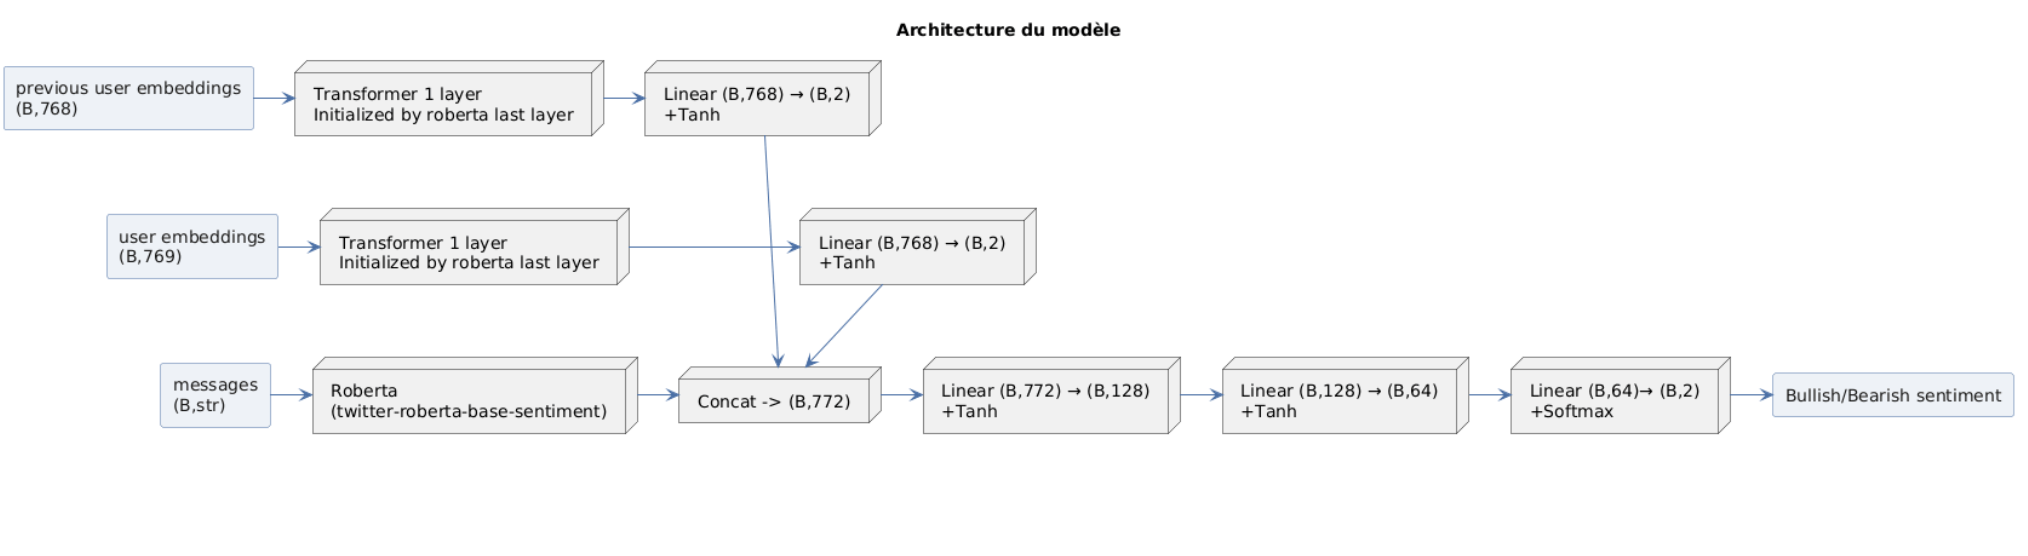
\includegraphics[width=1.1\textwidth]{schéma.png}
\caption{General diagram of the model with previous embedding and user embedding}
\end{figure}



\begin{table}[H]
\centering
\caption{Performances evaluated on 60000 tweets}
\begin{tabular}{lc}
\toprule
Model used & performances \\
\midrule
roberta + simple classification head & 83.14\% \\
adding user embedding & 88.24\% \\
adding previous embedding & 86.19\% \\
adding previous embedding and user embedding & 88.72\% \\
\bottomrule
\end{tabular}
\end{table}

In the case previous embedding + user embedding, we notice a significant gain for short messages (test on 15000 tweets): 

\begin{center}
\begin{tabular}{lcccc}
\toprule
 & T$\le$32 & 32$<$T$\le$64 & 64$<$T$\le$128 & 128$<$T$\le$256 \\
\midrule
roberta + simple classification head & 82.5\% & 88.0\% & 91.9\% & 91.1\% \\
adding user embedding & 88.9\% & 91.4\% & 89.4\% & 91.1\% \\
adding previous embedding & 86.6\% & 86.7\% & 88.6\% & 90.2\% \\
adding previous embedding and user embedding & 89.1\% & 89.6\% & 88.7\% & 90.3\% \\
\bottomrule
\end{tabular}
\end{center}
\\
On long tweets (which are much less numerous), we note a slight drop in performance with the addition of context (T<64) especially that of previous embedding (T<32). But the overall performance improves because the majority tweets have less than 32 tokens. If we took the max performances for each model, we see that we would reach 90\% overall ...

\section{Conclusion}
We can therefore have a very good prediction of tweets by taking into account the personality of the user and their previous tweets, even with ambiguous tweets. 

\section{Remaining points}

\begin{itemize}
\item  It would be interesting to provide the number of tokens to the model so that it learns to trust more the user embedding when it has enough tokens (and therefore use less the context information): With a little more time on this project, this would have been the next step.
\item  We could try to improve the handling of previous messages: tune the attention better
\item  Handle tweets that are replies, add the initial tweet in context
\item  It would be interesting to see if a user embedding remains credible for a long time if we do not update it 
\item  The hyperparameters of the network I created should be optimizable 
\item  Sometimes a model "collapses" at the beginning of training (even the simplest model with 1 classification head):
In that case, I restart and the shuffle does the job: I think that to stabilize learning it might be interesting to feed it at the beginning with tweets that are certainly non ambiguous.
\end{itemize}

\section{Public github repository}

\url{https://github.com/matthieubaucher/projet_NLP}


\end{document}
